\chapter{Application implementation}

\section{Backend server}

The backend server does not need to be particularly suited for large traffic or complexity. Its role is only to provide up-to-date GTFS data and manage user accounts. To this end, let's discuss about how it has been implemented.

As mentioned in the previous chapter, I used NestJS with TypeScript to build the backend server. NestJS is an opinionated framework that brings important abstractions (in the form of decorated classes and dependency injection) on top of an already-proven, battle-tested, HTTP server library (Express JS). NestJS can work with plain JavaScript, but augmenting it with TypeScript brings forth is fullest potential.

NestJS is heavily inspired from Angular, thus employs a system of \textit{modules}, that can be loaded into a Nest application individually, along with its dependencies, to the programmer's wish. Organizing into separate modules, or bundling everything into the default App module, is a decision taken by the programmer, taking into consideration applications such as microservices (different modules within the same project can be useful here) and complexity concerns (modules are hard to get to work). I chose to structure my project in modules that correspond to the following functionalities: authentication, GTFS file operation, user management.

\subsection{App module}
\label{sec:AppModule}

The App module is the big module that gets loaded and ran on application bootstrap. Presented in Figure \ref{FigBeBootstrap}, the application bootstrap code will initialize the Nest application using the \verb|AppModule| module as a root module, then takes some final steps in the setup of the environment, by disabling all CORS functionality and allowing all origins, allowing access to static assets (namely, the GTFS data, which is stored locally), and setting up the global \verb|ValidationPipe|, which takes care of request validation. When ready to listen to requests, we take the port from the environment (or use 3000 as default), then we start the Nest application.

\begin{figure}[htbp]
    \centering
    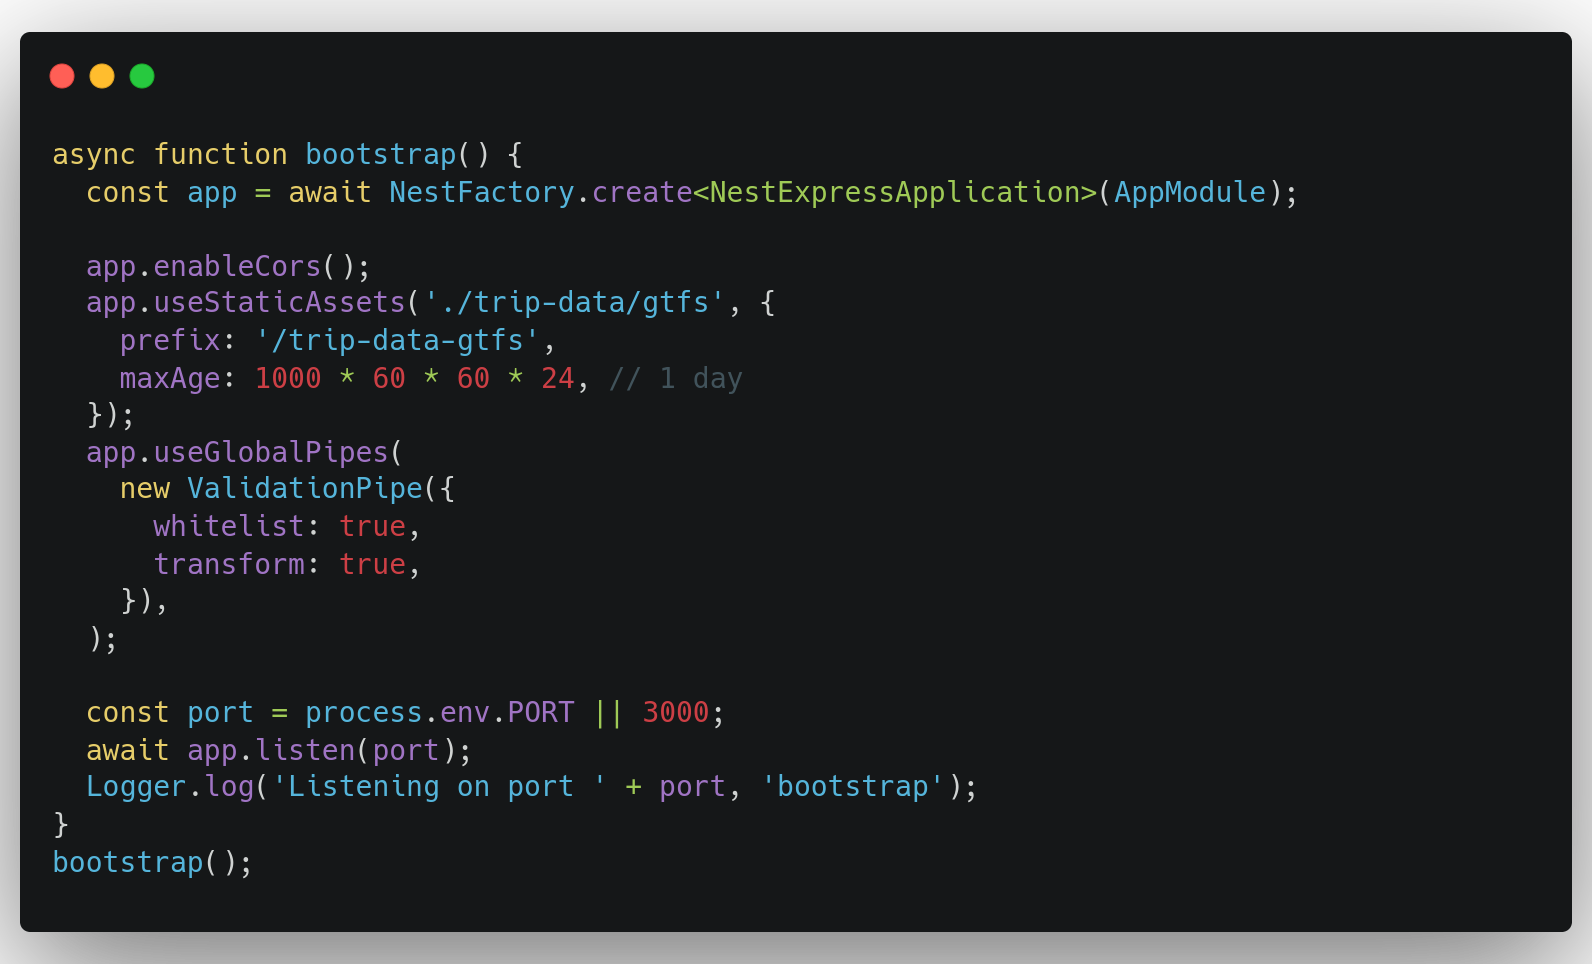
\includegraphics[width=0.9\textwidth]{./figures/code/be_bootstrap.png}
    \caption{Backend: bootstrapping code.}
    \label{FigBeBootstrap}
\end{figure}

Module definitions are not much more complex than importing all the dependency modules and adding them in the module definition, using the \verb|Module| decorator. The definition of the \verb|AppModule| is presented in Figure \ref{FigBeAppModule}, and consists of importing our three modules (auth, GTFS, and user) and the \verb|MongooseModule|, provided by Nest, which offers interaction with MongoDB databases, and the definition of the module class.

\begin{figure}[htbp]
    \centering
    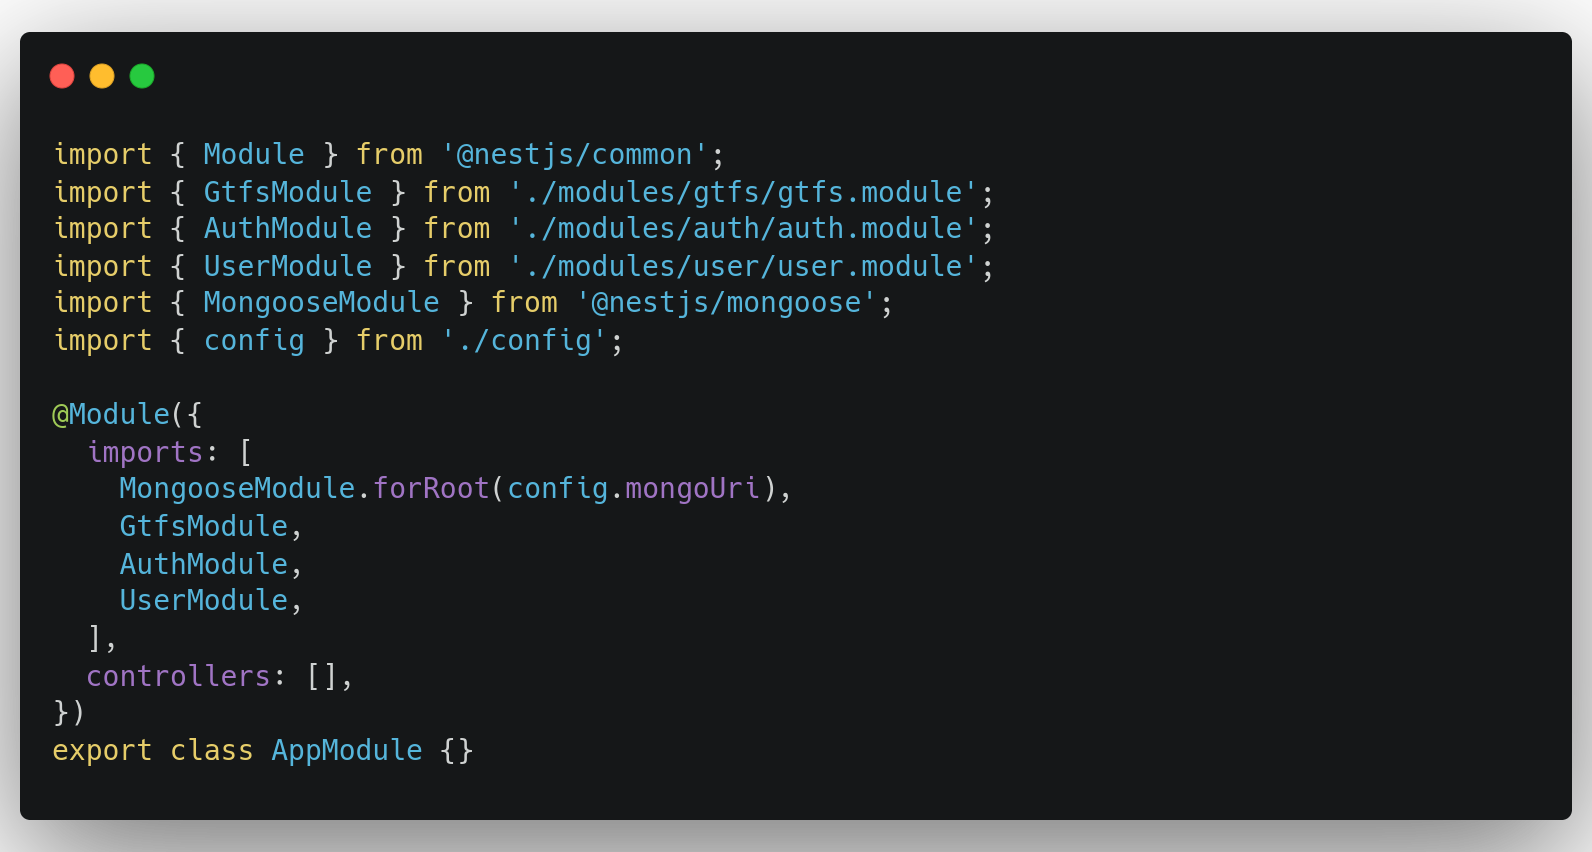
\includegraphics[width=0.9\textwidth]{./figures/code/be_app-module.png}
    \caption{Backend: AppModule.}
    \label{FigBeAppModule}
\end{figure}

\subsection{Configuration}
\label{sec:Configuration}

Backend configuration is stored in a \verb|config.yaml| file at the root of our project. The file is ignored by git, and serves as the location to place all the application secrets and connection instructions, along with configuration that might differ from an environment to the next.

A schema of the configuration file, without actual values, is presented in Figure \ref{FigBeConfig}. We can see configuration related to GTFS (where to download GTFS data from, and what files), along with social authentication secrets, MongoDB database URL, and JWT generation secret.

\begin{figure}[htbp]
    \centering
    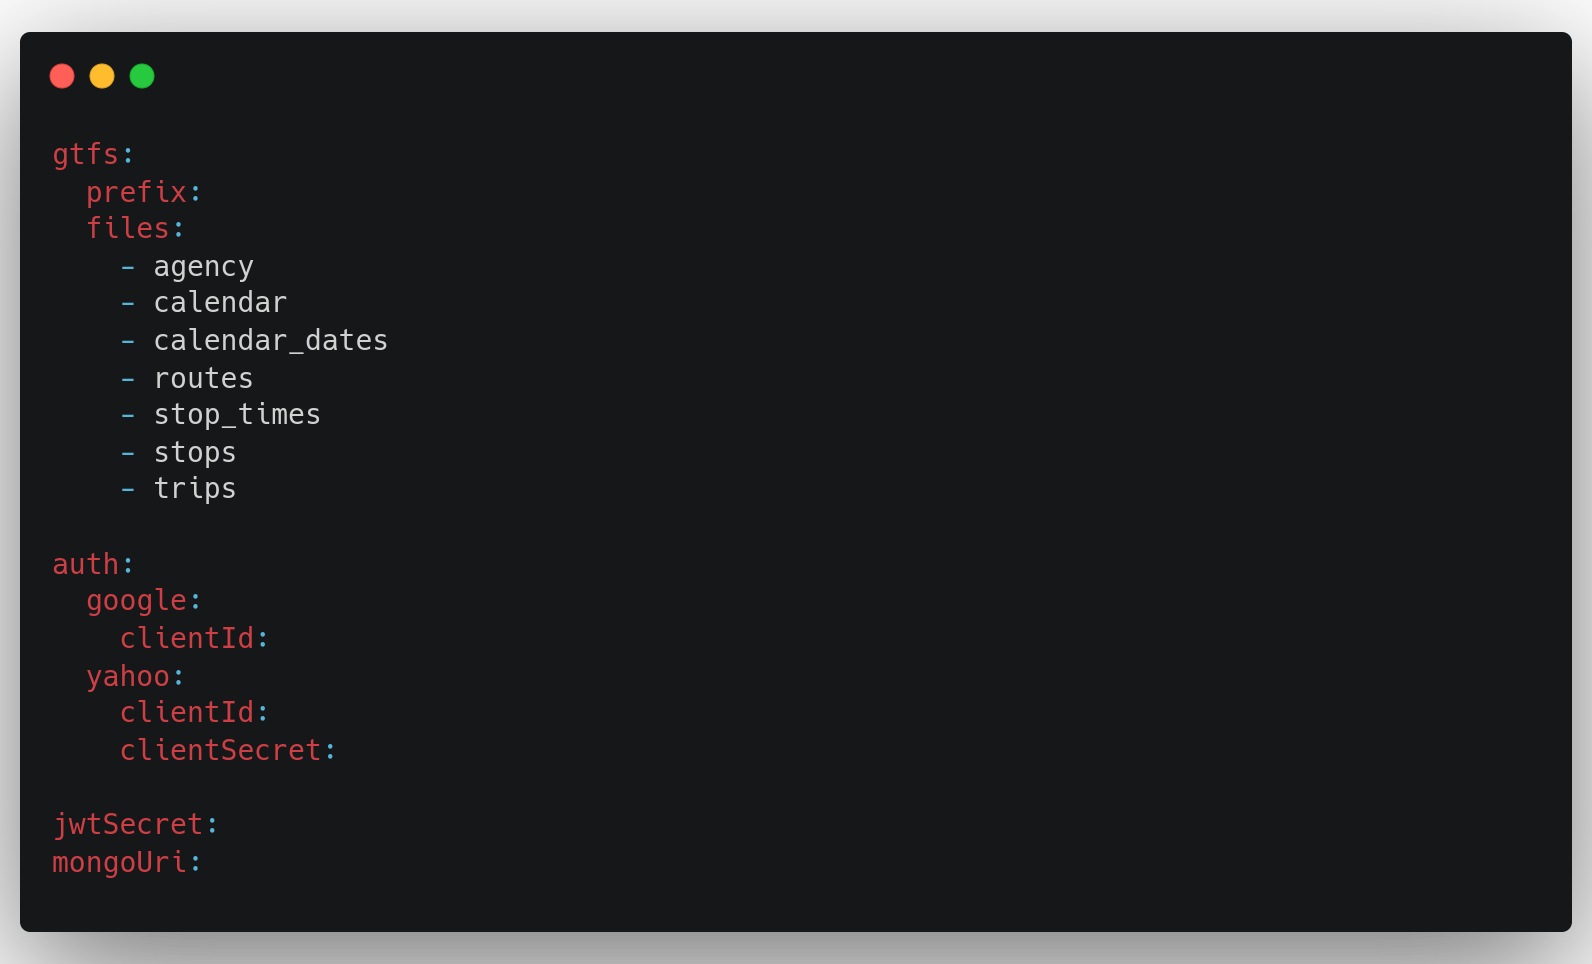
\includegraphics[width=0.9\textwidth]{./figures/code/be_config.png}
    \caption{Backend: config.yaml}
    \label{FigBeConfig}
\end{figure}

The YAML file is then loaded into memory in the \verb|config.ts| TS module, then exported so that it is available for the entire application.

Having the configuration file be loaded by Node is a decision taken in light of simplicity. NestJS offers ways of integrating configuration within its module system, but it requires writing additional code and logic, not only for the providing module, but for modules and services that use the configuration too.

As a safety precaution, the config file is validated against a schema using Joi, which can help identify missing configuration parameters at application startup, rather than have the application crash when it tries to access an inexistent configuration parameter. The Joi schema is presented in Figure \ref{FigBeConfigSchema}.

\begin{figure}[htbp]
    \centering
    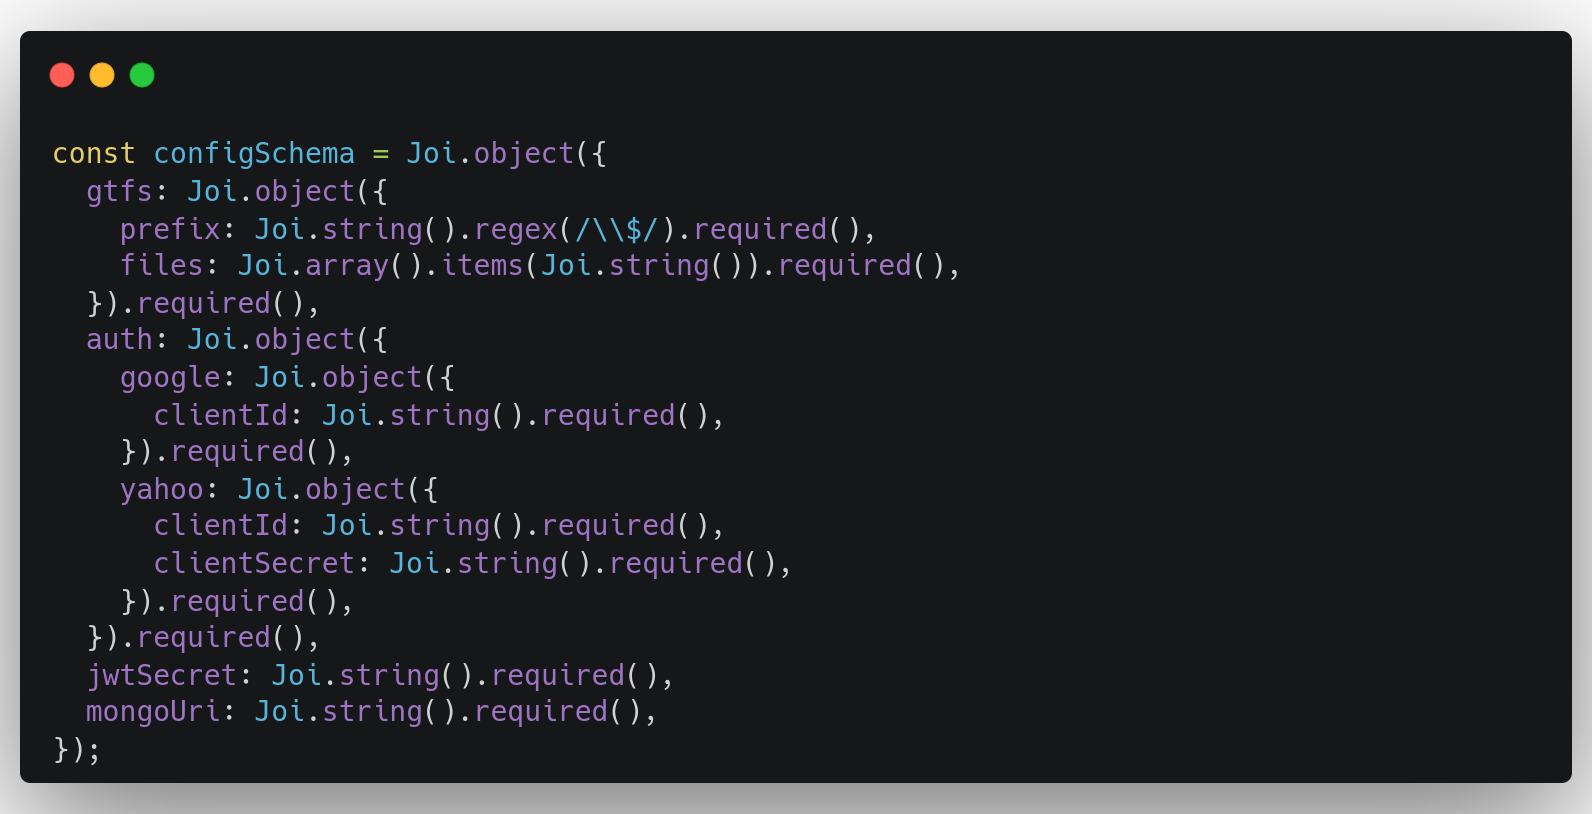
\includegraphics[width=1\textwidth]{./figures/code/be_config-schema.png}
    \caption{Backend: config validation schema.}
    \label{FigBeConfigSchema}
\end{figure}

\subsection{Preparing GTFS data for download}

The GTFS files are available on Vasile Coțovanu's GitHub repository \cite{VasileRubyExporter}, and before serving to our frontend, the files need to be downloaded locally first.

To this end, there exists a script called \verb|process-gtfs.ts|, that when run, creates a Nest application but only loads the GTFS module (Figure \ref{FigBeGTFSBootstrap}). The script then retrieves the \verb|GtfsService| service and uses it to initiate the download of GTFS data from GitHub, which is then placed in the \verb|trip-data| directory. This directory is then referenced in the static assets declaration from the application bootstrapping code (see Section \ref{sec:AppModule}).

\begin{figure}[htbp]
    \centering
    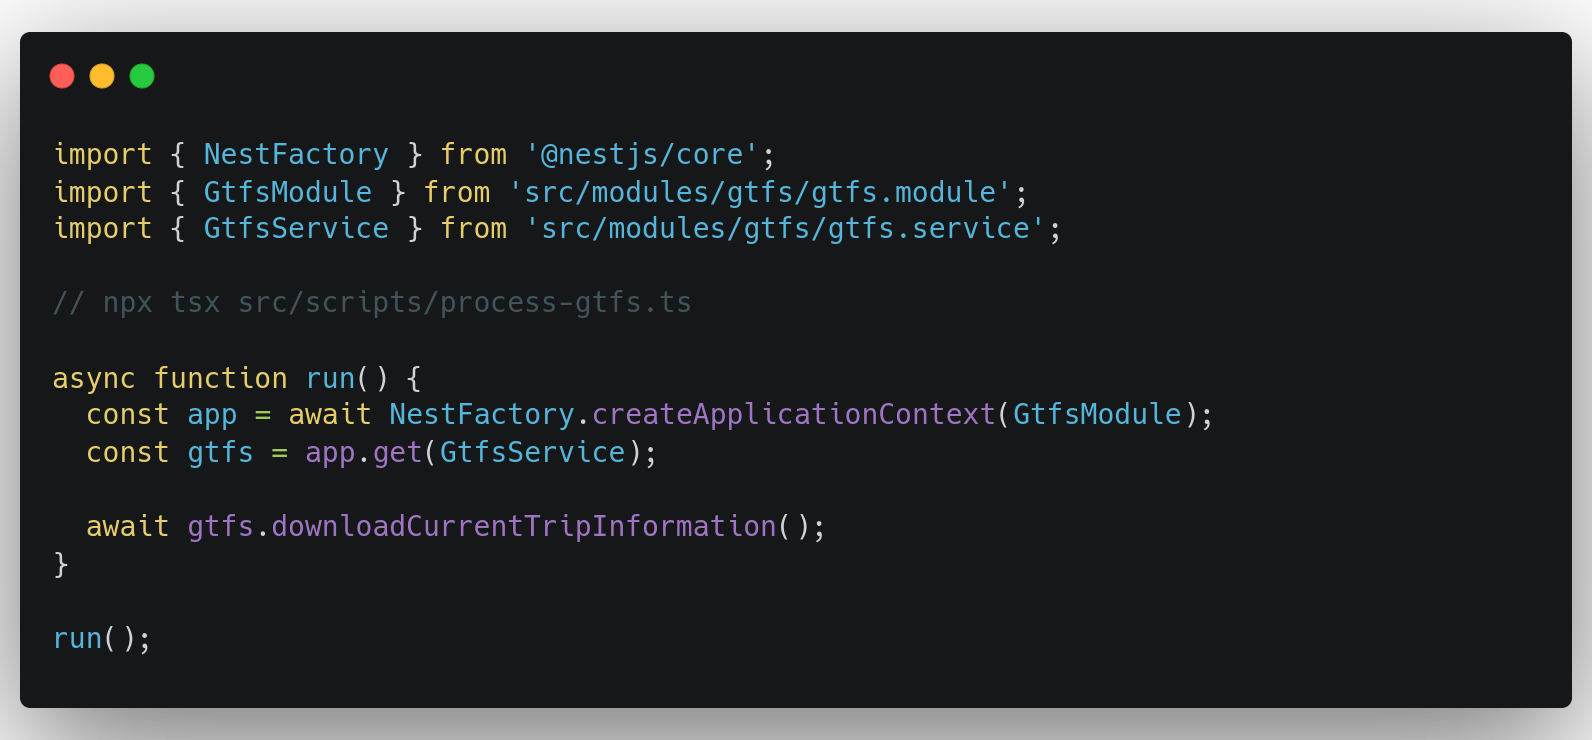
\includegraphics[width=1\textwidth]{./figures/code/be_gtfs-bootstrap.png}
    \caption{Backend: GTFS script bootstrapping code.}
    \label{FigBeGTFSBootstrap}
\end{figure}

\subsection{Auth module}

\begin{figure}[htbp]
    \centering
    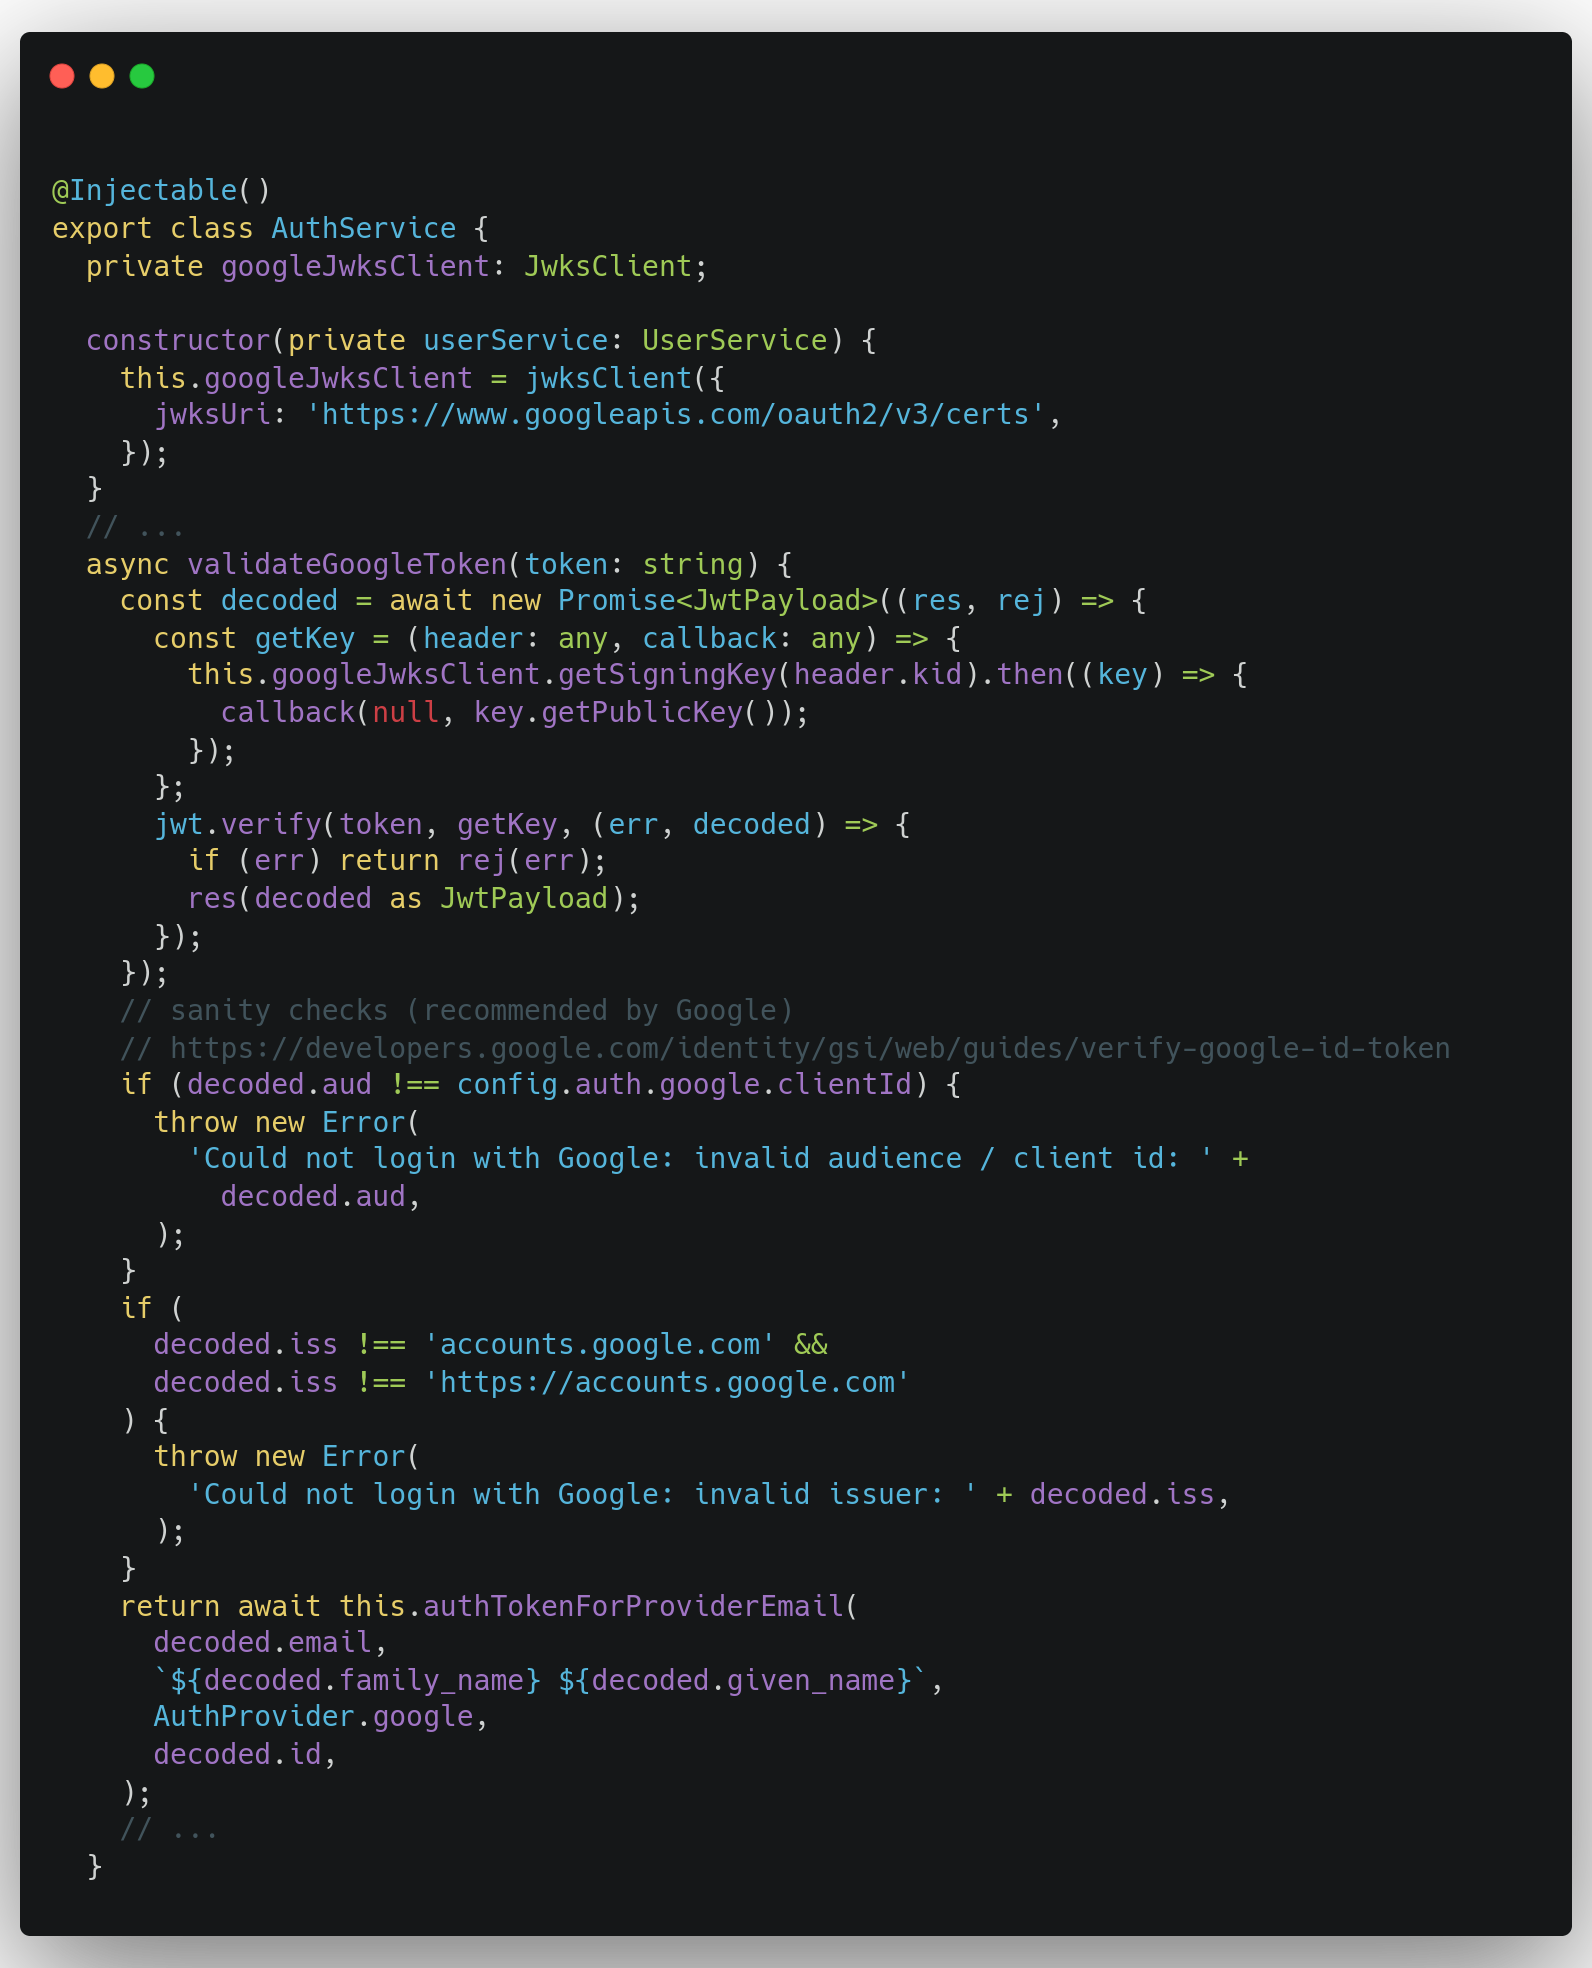
\includegraphics[width=0.9\textwidth]{./figures/code/be_auth-service-google.png}
    \caption{Backend: code that validates Google JWT tokens, for Google sign-in.}
    \label{FigBeAuthServiceGoogle}
\end{figure}

The Auth module has functionality related to user authentication: validating social logins, validating username and passwords, generating JSON Web Tokens (JWTs) and validating those tokens.

Google Sign-in is validated using a token received from the frontend and emitted by Google. The token is a JWT that is encoded using a JSON Web Key (JWK). Google publishes the public keys they use in a JSON Web Key Set (JWKS) format, which can be used to validate JWT tokens emitted from them, and verify their authenticity. Google also recommends performing a set of sanity checks on the JWTs apart from checking their signature, to prevent various attacks, such as emitting valid JWTs for a different application, or from a different Google service. The JWT signature verification library used in the app also makes sure that \verb|iat| and \verb|exp| are enforced (disallowing expired tokens). See Figure \ref{FigBeAuthServiceGoogle} for a code snippet of this step.

Yahoo Sign-in is validated by redirecting the user through a traditional OAuth authorization flow. At the end of the frontend flow, the backend receives a code that will then be sent to Yahoo (using a REST API) for validation, resulting in an \verb|access_token| that grants permission to Yahoo's OAuth APIs. The backend then makes a request to the userinfo endpoint, retrieving the user's email.

Upon validating social credentials, the backend then checks for an user account that already exists in the database (matching using the user's email as received from the social provider), creating one if one doesn't already exist. For this user id, a JWT token is emitted using the application secret (as defined in the configuration, see Section \ref{sec:Configuration}), and returned to the frontend.

The \verb|AuthModule| also provides methods to verify user JWTs, and a Request Guard that can be used to guard API routes that require authentication. Validating JWTs from API requests is done via a library called \verb|passport| and its Nest integration \verb|@nestjs/passport|. Making use of the JWT passport strategy, we can easily configure a strategy that checks JWTs received in the \verb|Authorization| header, via the application's JWT secret. The code is available in Figure \ref{FigBeJwtStrategy}, where it can be noticed how we configure \verb|passport| to validate JWTs, and tell it how to retrieve a user from a valid JWT by making use of the \verb|AuthService|.

\begin{figure}[htbp]
    \centering
    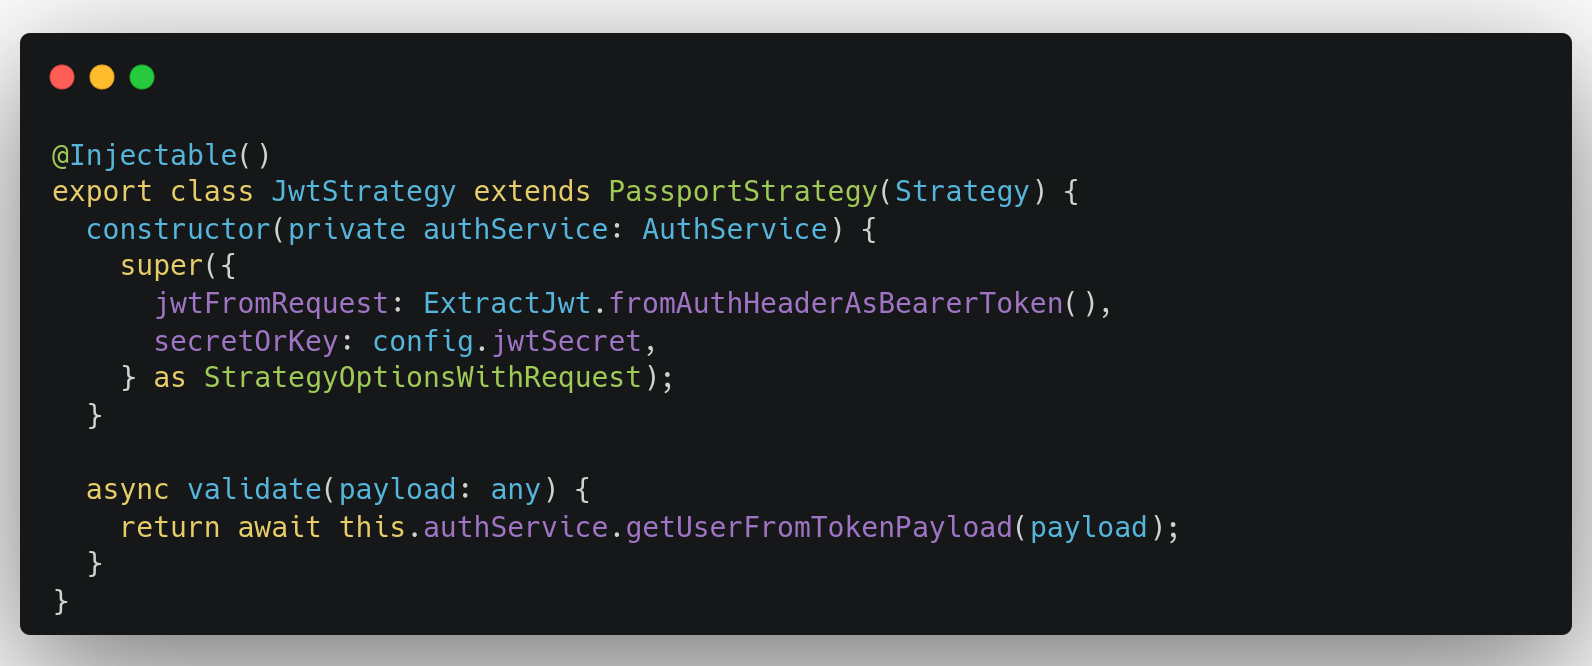
\includegraphics[width=1\textwidth]{./figures/code/be_jwt-strategy.png}
    \caption{Backend: the JWT strategy, as defined using @nestjs/passport.}
    \label{FigBeJwtStrategy}
\end{figure}

A popular method of accessing user data pertaining to a request, in the Express framework, is by attaching a \verb|user| property on the \verb|req| (Request) object. This object is passed around to all handler code in the app, making it an easy way of passing request state around the application. Nest abstracts away this \verb|req| object, and although it provides ways of accessing it, they are discouraged in lieu of a more opinionated approach, that is less prone to type errors. The Nest approach of decoding the user from the request consists of creating a decorator that makes this decoding for us, and places the user object into a parameter of choice in the controller code. The definition of this decorator, along with an example, is shown in Figure \ref{FigBeReqUser}.

\begin{figure}[htbp]
    \centering
    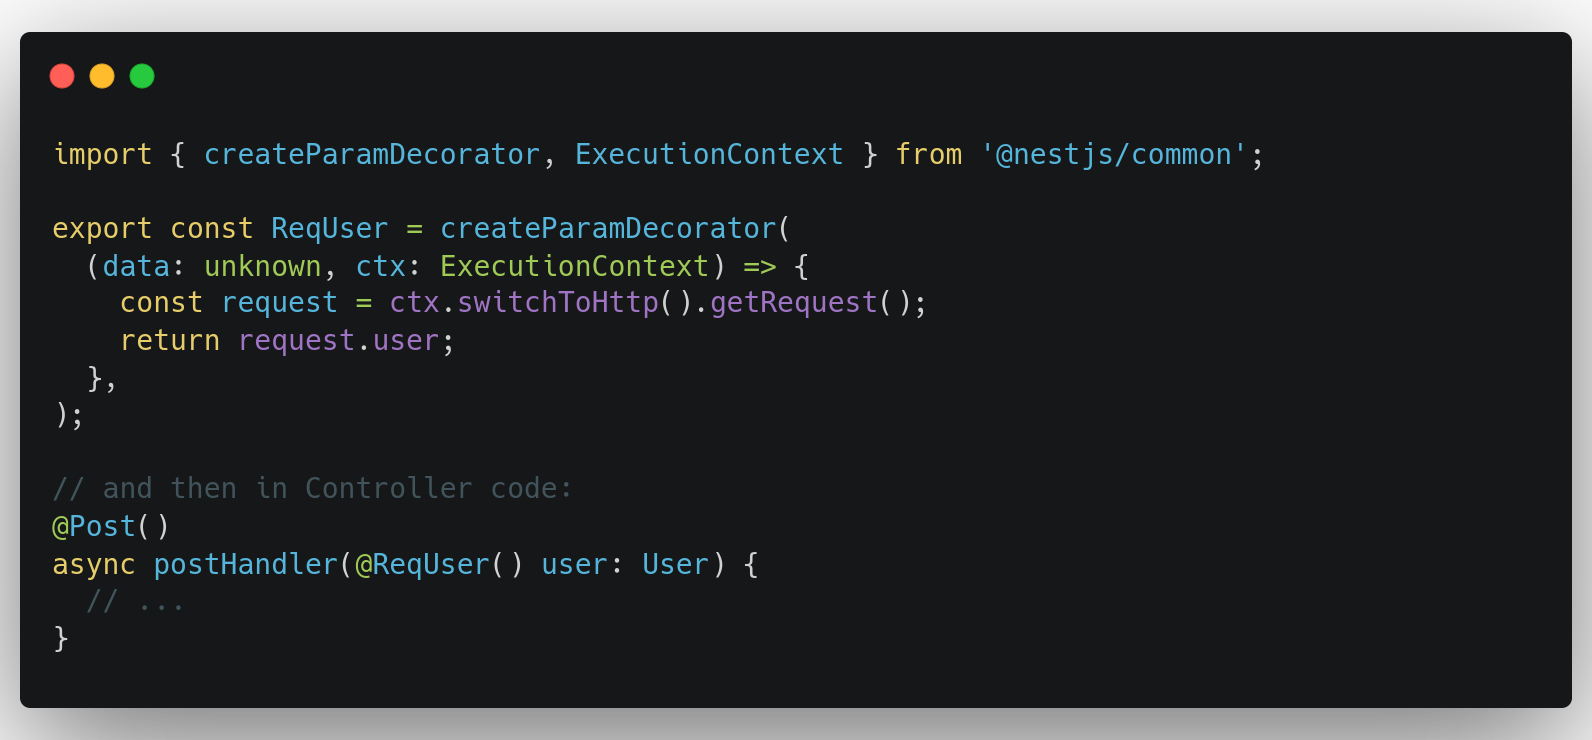
\includegraphics[width=1\textwidth]{./figures/code/be_req-user.png}
    \caption{Backend: the definition of the @ReqUser() decorator, along with an usage example.}
    \label{FigBeReqUser}
\end{figure}

\subsection{DTO validation}

All request validation throughout the app is performed using Data Transfer Objects (DTOs), that are decorated with specific validation criteria.

\begin{figure}[htbp]
    \centering
    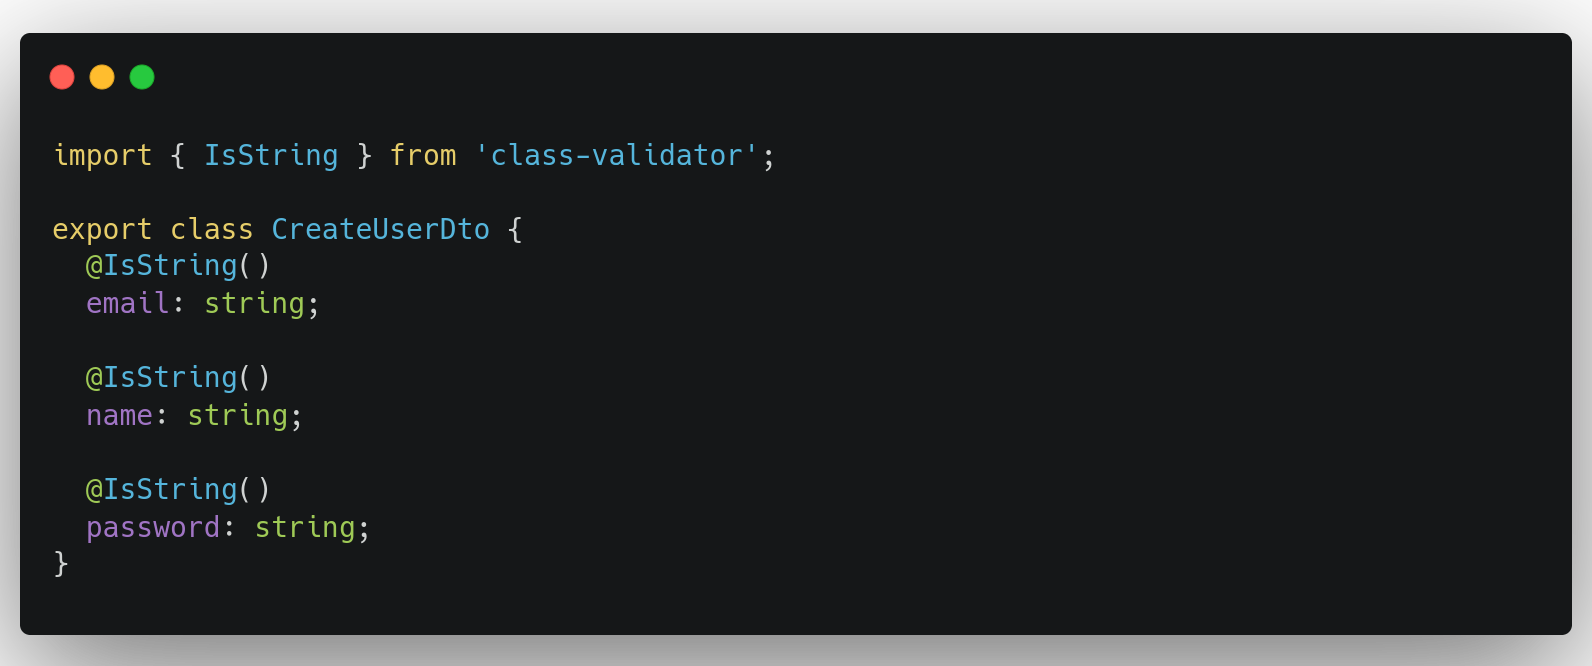
\includegraphics[width=1\textwidth]{./figures/code/be_dto.png}
    \caption{Backend: the definition of a DTO with validation, exemplified on the register request.}
    \label{FigBeDto}
\end{figure}

Figure \ref{FigBeDto} shows how such a validation class looks like. The \verb|ValidationPipe| declared globally (referenced in Section \ref{sec:AppModule}) will use this class decorated with \verb|class-validator| validators to validate the request body of the register endpoint. If a property is found to have a different type to the one specified in the constraint, \verb|class-validator| will throw an error and Nest will return a HTTP 422 status code, with detailed information about how the payload is malformed.

You can notice that the class fields are annotated with TypeScript types (in this case, string). It is important to point out that these types are not enforced at runtime, since they only aid in compile-time type safety. There is nothing to prevent the programmer from adding TS types here that do not match with the decorators, however this mistake is unlikely due to how the decorators are placed right next to the properties.

A special kind of attack can be performed by adding more properties on the request body object that have special significance to other components of the application (for example, MongoDB). By default, the ValidationPipe provided by Nest only checks that those three fields (email, name, password) are valid, but once these checks are complete, the entire request body is deserialized and converted into a JS object, with all its properties. It's then trivial for those properties to be passed to \verb|mongoose| database code, as a byproduct of language features such as the spread syntax (\verb|...obj|), and then have them run arbitrary queries on the database system. To this end, the ValidationPipe offers a configuration parameter \verb|whitelist|, that will remove all extraneous properties that are not explicitly validated in the DTO. If unvalidated properties are desired, the programmer can use the \verb|@Allow()| decorator.

\subsection{User module}
The user module handles users and their trips. The trips are not separated in another module due to how they are stored in the database under the same document, and thus are accessed using the same MongoDB collection (or model, as described by \verb|mongoose|).

\begin{figure}[htbp]
    \centering
    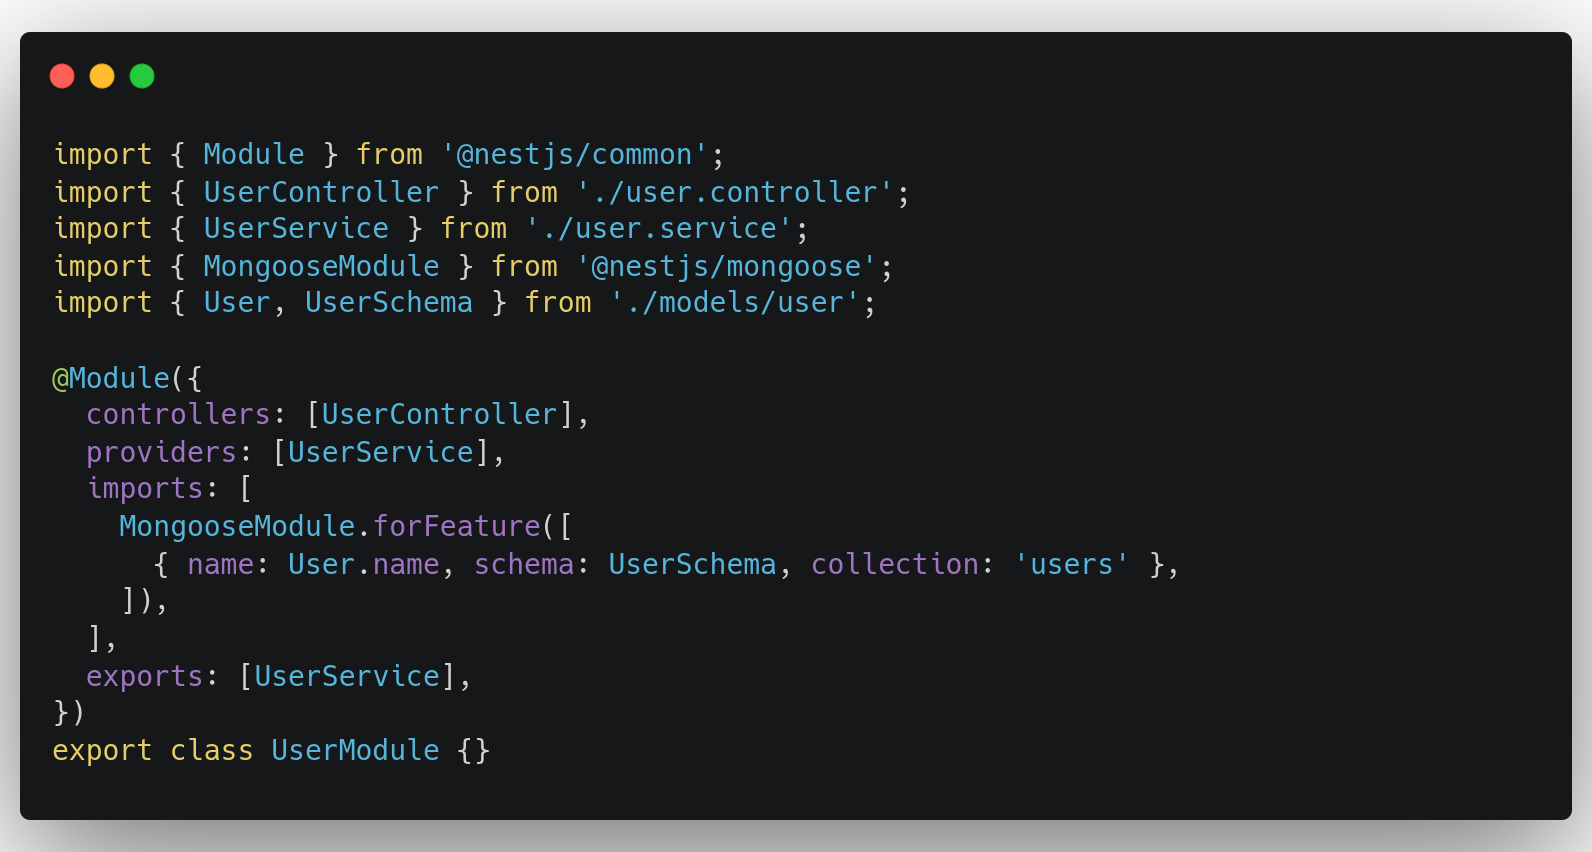
\includegraphics[width=1\textwidth]{./figures/code/be_user-module.png}
    \caption{Backend: the user module.}
    \label{FigBeUserModule}
\end{figure}

Figure \ref{FigBeUserModule} shows the definition of the UserModule. It is interesting to notice the separate parts of the module declaration:
\begin{enumerate}
    \item \textbf{controllers:} represents the list of controllers that this module exposes to the Nest framework. Controllers that are not registered here are not visible to Nest's internal router.
    \item \textbf{providers:} represents the list of providers that this module makes use of. A provider is any class decorated with \verb|@Injectable()|, and all providers are available for dependency injection.
    \item \textbf{imports:} represents a list of modules that this module depends on. Namely, we depend on MongooseModule. However, registering MongooseModule as a root module is not suitable here, since we already imported it as root in AppModule. For this reason, we use \verb|.forFeature()|, which is used to register specific models for use with \verb|mongoose|.
    \item \textbf{exports:} represents a list of all providers that this module exposes to other modules. As a consequence, all modules that import UserModule have access to the UserService. The module that makes use of this service is the AuthModule.
\end{enumerate}

Another interesting analysis we can make is on the User model. The \verb|mongoose| framework makes use of \textit{schemas} to enforce object validation on the documents that get persisted to the database. However, the schemas need to be declared in plain JavaScript, and since they don't integrate well with TypeScript, the mongoose documentation recommends writing the schema twice: once for registering in mongoose, and once for TypeScript type safety.

Nest offers native support for mongoose, and comes with a solution to enable a single class to provide both a mongoose schema, and TypeScript type safety. Visible in Figure \ref{FigBeUserModel}, the solution consists of decorating all class properties using the \verb|@Prop()| decorator, in a manner not unlike the validation performed by the validation library \verb|class-validator|.

All the \verb|@Prop()| arguments are directly passed to mongoose, so as to make the abstraction as minimal as possible. Similarly, all arguments to \verb|@Schema()| are passed to the mongoose Schema constructor.

In this manner, the class is already ready for TypeScript, and only awaits conversion to a mongoose Schema with the Nest \verb|SchemaFactory.createForClass()| method, seen in action in the last line of Figure \ref{FigBeUserModel}.

\begin{figure}[htbp]
    \centering
    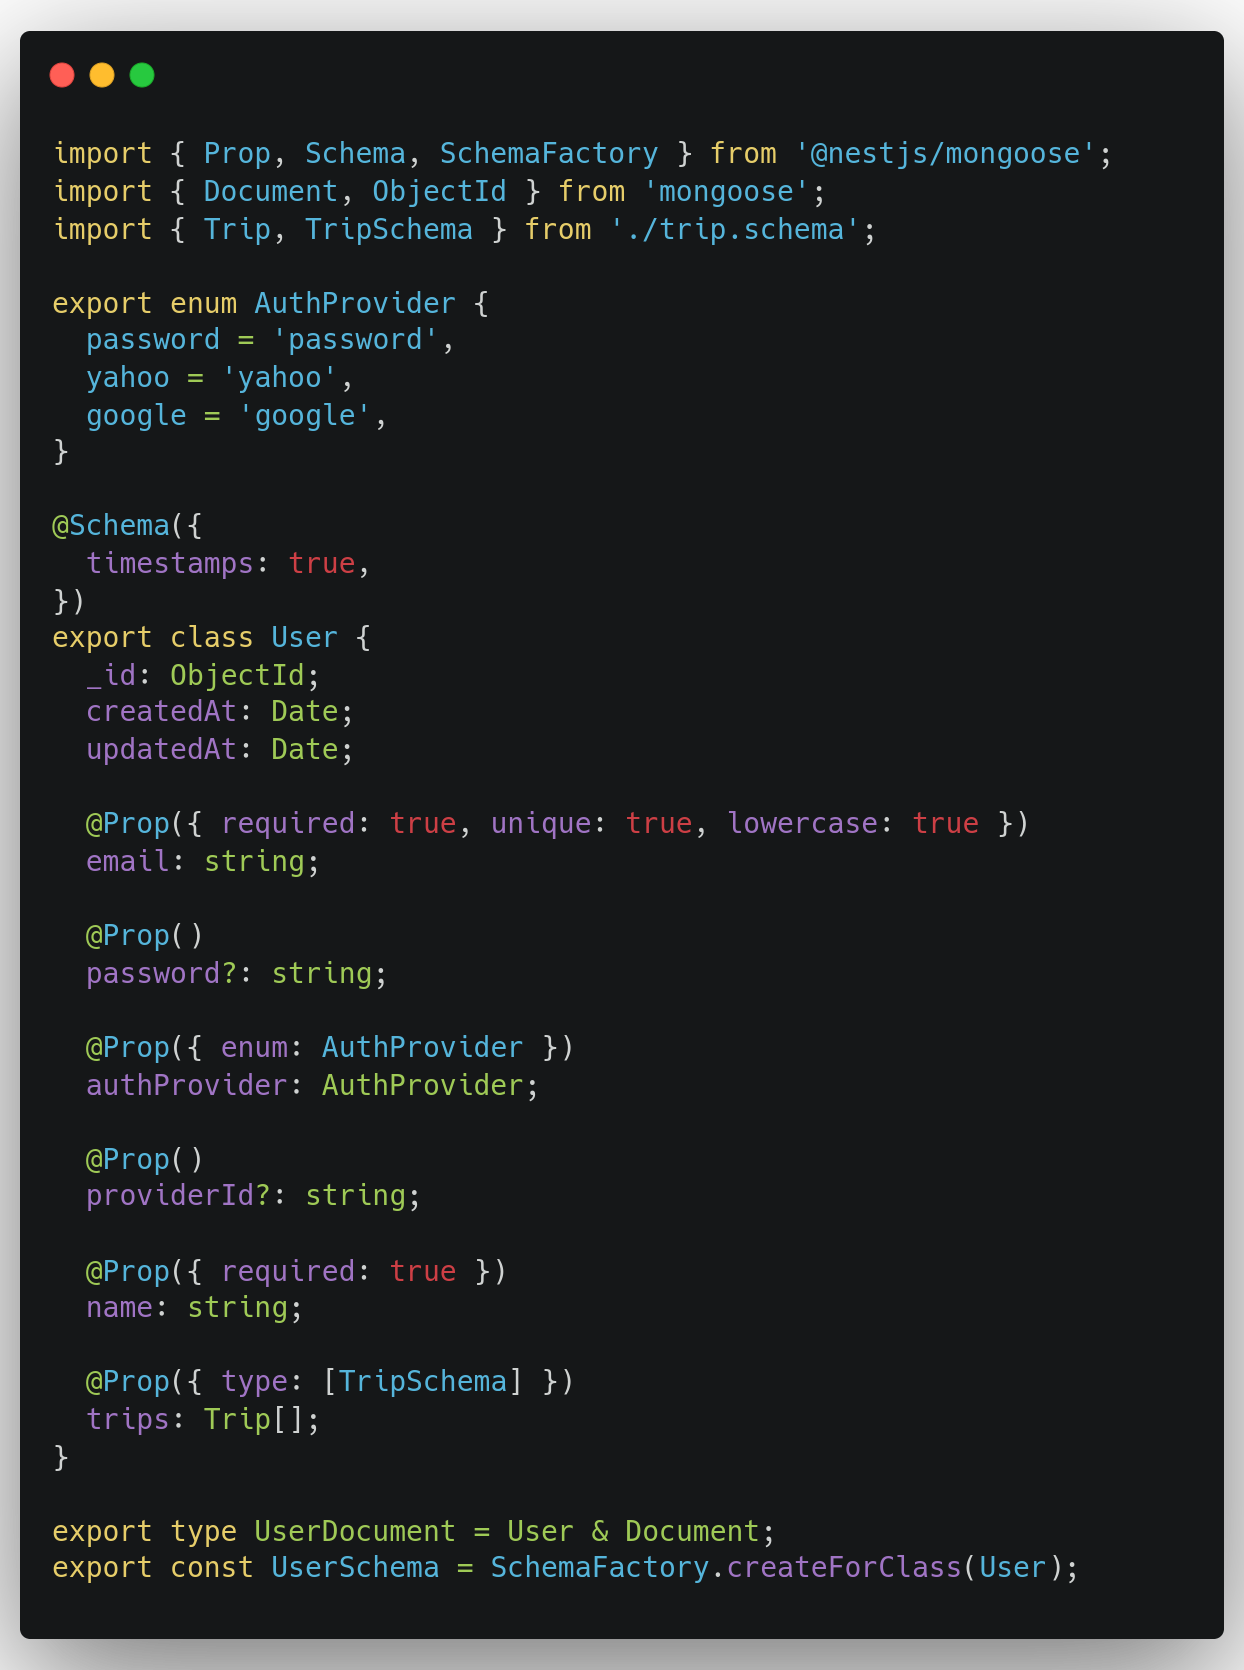
\includegraphics[width=.8\textwidth]{./figures/code/be_user-model.png}
    \caption{Backend: the user model.}
    \label{FigBeUserModel}
\end{figure}

\subsection{Building the project}

Since we employed TypeScript in the project, we are now required to compile the project in order to make it runnable. Albeit running the project directly (the TS files) is possible using tools such as \verb|ts-node| or \verb|tsx|, these tools compile the code on-the-fly, thus making the overall execution slower.

This being said, the compilation does not involve any additional steps apart from the TypeScript compilation.

As such, compiling the project is as easy as running \verb|npm run build| from the root directory of the project. This compiles all TS code and outputs it in the \verb|dist| directory. One can now run \verb|dist/index.js| directly, or use \verb|npm start|, to start the server.

\subsection{Deployment of the backend}
Deployment of the backend infrastructure is an interesting case study.

For one, a happy consequence of having the database deployed in the cloud separately is how we don't need to create any special infrastructure for it, since just passing the correct connection URL to the backend application is sufficient for it to successfully connect to it. The database connection is sufficiently fast, even across the Internet (as opposed to on the local computer or even network), as long as the backend and frontend are roughly in the same geographic region (eg. Frankfurt, where both DigitalOcean and Atlas have data centers).

For another, there are cost restrictions imposed on the deployment. I personally own a DigitalOcean droplet (virtual machine in the cloud) that I use for all my projects, so as to have a fixed monthly costs regardless of traffic.

As such, the steps I use to deploy the backend is as follows:
\begin{enumerate}
    \item If first time, clone the repository on the remote machine. Otherwise, just git pull.
    \item Run \verb|npm i| to download or update dependencies.
    \item If first time, make sure the \verb|config.yaml| configuration is suited for production.
    \item Build the project.
    \item If first time, create a \verb|ecosystem.config.js| file, telling PM2 how to run my app (see Figure \ref{FigBeEcosystemConfig}). PM2 is the process manager I use on the VM, that handles app restarts, logs and monitoring.
    \item Run the project using PM2, letting it take over.
\end{enumerate}

\begin{figure}[htbp]
    \centering
    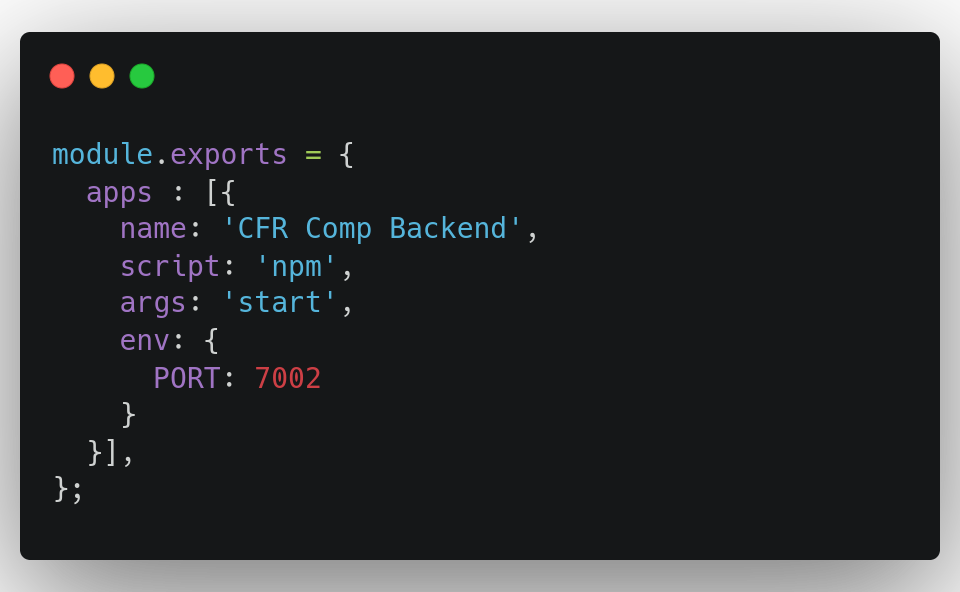
\includegraphics[width=.8\textwidth]{./figures/code/be_ecosystem-config.png}
    \caption{Backend: the ecosystem config, used by PM2 on my personal VM instance.}
    \label{FigBeEcosystemConfig}
\end{figure}

Having a shared virtual machine as a deployment environment proves a challenging task for any continuous integration / continuous development pipelines setup. For this task, I used an application specifically to handle this odd deployment scenario, called Deploy Monkey, available on GitHub \cite{DeployMonkey}. This custom application can link GitHub Actions (by use of webhooks) with my droplet, such that my droplet can automatically run the steps defined above locally, upon notification from GitHub that a push happened.

\section{Frontend application}
Arguably the most important part of the application, the frontend is written in React with TypeScript and is written to be conformant to the PWA specification, so that it possesses the qualities of a PWA: installable and functional offline.

The bundler used is Vite. The role of a bundler is to take all the different source files and "bundle" them together in a single monolithic file, while also passing the code through all the required compilation steps. In this case, Vite also offers features to help with the development experience, such as hot reloading, and a local web server.

For our purposes, Vite also offers a plugin that helps us convert our application into a Progressive Web Application.